\documentclass[a4paper,11pt]{scrartcl}

\usepackage{graphicx}
\usepackage[utf8]{inputenc} 
\usepackage{amsmath,amssymb,amsthm} 
\usepackage[round]{natbib}
\usepackage{url}
\usepackage{xspace}
\usepackage[left=20mm,top=20mm]{geometry}
\usepackage{algorithmic}
\usepackage{subcaption}
\usepackage{mathpazo}
\usepackage{booktabs}
\usepackage{hyperref}
% \usepackage{draftwatermark}

\newcommand{\ie}{ie}
\newcommand{\eg}{eg}
\newcommand{\reffig}[1]{Figure~\ref{#1}}
\newcommand{\refsec}[1]{Section~\ref{#1}}

\setcapindent{1em} %-- for captions of Figures

\renewcommand{\algorithmicrequire}{\textbf{Input:}}
\renewcommand{\algorithmicensure}{\textbf{Output:}}


\title{Documentation Notes}
\date{}
\author{Giuseppe Cervone\\ \url{giuseppe.cervone@edu.unife.it}}

\begin{document}

\maketitle

\section{Devices}

\section{Materials used}
The aim of the project is to develop what in cybersecurity it's called a data diode, a unidirectional communication device for data exchange. The importance behind this project is that industrial data diodes are expensive devices, and implementing a high amount of them like for this specific use case is a very costly move, but with software implementations (firewalls) or hardware implementations (serial or optical communications) it is possible to have cheaper data diodes that are almost as functional for most use case scenario. The setup will include two Raspberry Pi model 3 with a specific configuration which we will highlight later, and a TTL-232R-3V3 cable without the RX pin.
\subsection{Raspberry Pi}
The machines are configured as follows:
\begin{itemize}
    \item Raspberry Pi 3 Model B Ver1.2:
    \begin{itemize}
        \item Quad Core 1.2GHz Broadcom BCM2837 64bit CPU
        \item 1GB RAM
        \item BCM43438 wireless LAN and Bluetooth Low Energy (BLE) on board
        \item 100 Base Ethernet
        \item 40-pin extended GPIO
        \item 4 USB 2 ports
        \item 4 Pole stereo output and composite video port
        \item Full size HDMI
        \item CSI camera port for connecting a Raspberry Pi camera
        \item DSI display port for connecting a Raspberry Pi touchscreen display
        \item Micro SD port for loading your operating system and storing data
        \item Upgraded switched Micro USB power source up to 2.5A
        \item Raspberry Pi OS Lite
        \item 16GB microSD card
    \end{itemize}
\end{itemize}

Using the RPI-Imager tool I installed the latest Raspberry PI OS image. Upon first boot up, remember that raspberry pi login is username: pi, password: raspberry. As Raspberry Pi OS Lite is an OS without a desktop environment, so we can use raspi-config to enable a series of features useful for testing software:
\begin{itemize}    
    \item In the system options:
    \begin{itemize}
        \item Enable WIFI
        \item Change username and password if needed
        \item Change hostname to whatever it's preferred. This is useful in the future to enable SSH
    \end{itemize}
    \item In the interface options:
    \begin{itemize}
        \item Enable SSH
        \item Enable Serial interface, remembering to disable login shell but enable serial interface.
    \end{itemize}
    \item Run sudo apt-get upgrade to make sure all packages are up to date before using raspi-config
    \item In my config the SSH internal ip's should be:
    \begin{itemize}
        \item ssh pi@192.168.1.157 RX
        \item ssh pi@192.168.1.198 TX
        \item password raspberry
    \end{itemize}
\end{itemize}

Having the machines setup, I moved on to the first test, sending an "Hello, World!" from Raspberry 1 to Raspberry 2. I will be starting with a serial communication via a TTL-232R-3V3 cable, which is USB to UART, with +3.3V TTL levels UART signals. The cable has 3-pins on one end, and USB on the other. Using GPIO14 pin on the RPi we can trasmit data, using GPIO15 we receive data. 
Beow we can see from the documentation of the cable the correct way to plug in the various cables in the correct pins.
\begin{figure}[htbp]
\centerline{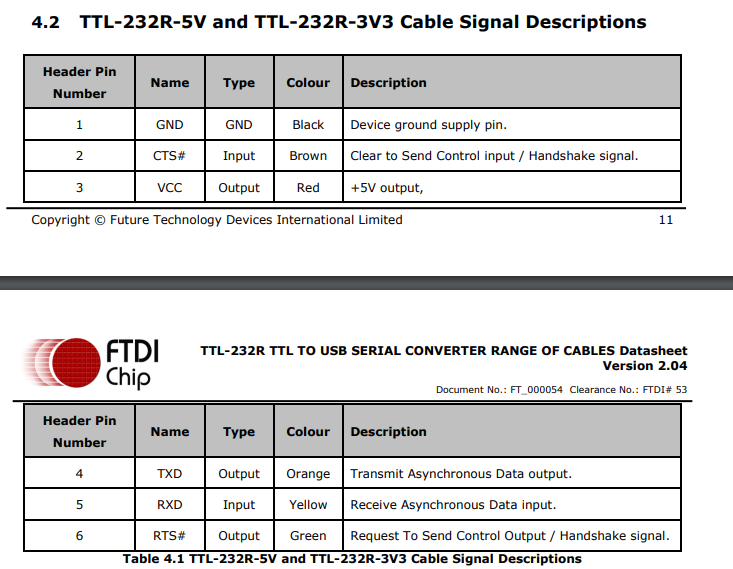
\includegraphics{pinout uart.png}}
\caption{Pinout del cavo seriale}
\label{fig2}
\end{figure}

With the cable plugged in we run the command ls /dev/tty* on both raspberry machines so we have an idea of what port we are using on each raspberry in the serial communication (For the port that's sending data it should be /dev/ttyS0, while for the other port it should be USB0).

The first implementation of a data diode I will try out is a project based on a github repo that is not mantained anymore. https://github.com/thephez/data-diode.

Here below is an image of what I will try to implement in this version 0.0.1.
\begin{figure}[htbp]
\centerline{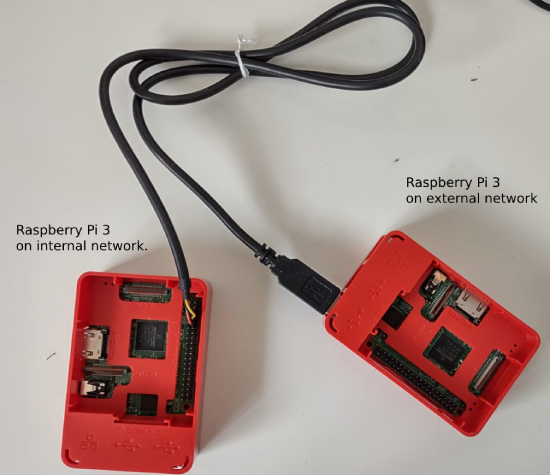
\includegraphics{0.0.1.png}}
\caption{Versione 0.0.1}
\label{fig}
\end{figure}



\bibliographystyle{plainnat}
\bibliography{/Users/hugo/references/references}

\end{document}
l
